\chapter{Quando la legge di Moore volge al termine}
\fancyhead[RO, LE]{\bfseries Quando la legge di Moore volge al termine}
In questo capitolo si vogliono introdurre due tipologie di computer, a partire da quello moderno che tutti noi conosciamo fino ad arrivare alla nascita di quello quantistico, mettendo in evidenza l'importanza del suo sviluppo.


\section{I computer classici}
\textit{Un computer è una macchina automatizzata che svolge due operazioni fondamentali: effettua complessi calcoli matematici ed elabora informazioni; spetta quindi al programmatore impartire ordini all'elaboratore per risolvere determinate problematiche \cite{computer2004articolo}.}

Le prime informazioni e testimonianze storiche a noi note riguardanti gli algoritmi di calcolo sono molto antiche, per avere una definizione formale di algoritmo si è dovuto attendere sino agli anni '30, dove in maniera indipendente, Alonzo Church ed Alan Turing si impegnarono nella risoluzione di un problema posto da David Hilbert qualche anno prima.
La questione su cui si interrogò riguardava l'esistenza di algoritmi capaci di risolvere ogni problema della matematica, introducendo così il concetto di problema decisionale.

Fu Turing che nel 1936, dopo aver pubblicato un articolo teorico, sviluppò un modello per la computazione in grado di eseguire algoritmi, chiamato macchina di Turing \cite{turing1936articolo}.
Quest'ultimo diede poi luogo allo sviluppo dell'attuale computer moderno e successivamente dimostrò anche l'esistenza di una macchina di Turing universale, la quale poteva essere usata per simulare le operazioni svolte in una qualsiasi macchina di Turing.

Dato quindi un algoritmo eseguibile su qualsiasi hardware, esiste il suo equivalente per una macchina di Turing universale che esegue lo stesso esatto compito.
Il concetto di \say{efficienza} \cite{dipierro2013articolo} di un algoritmo ci permette di capire meglio i vantaggi della computazione quantistica, che espressa in termini matematici nella teoria della complessità computazionale può essere riassunta brevemente come segue: un algoritmo è efficiente se il tempo di esecuzione è una funzione polinomiale rispetto alla grandezza del problema risolto (o lunghezza dell'input); un algoritmo è inefficiente se il tempo di esecuzione è superiore al polinomiale (tipicamente esponenziale).

Alla fine degli anni '60 e all'inizio degli anni '70 venne introdotta la tesi di Church-Turing i quali affermavano di poter simulare efficientemente su di una macchina di Turing un qualsiasi processo algoritmico.

Con l'aumentare della potenza degli hardware in maniera esponenziale, Gordon Moore nel 1965 codificò questa crescita attraverso la legge di Moore:
\begin{center}
\textit{\say{La complessità di un microcircuito, misurata ad esempio tramite il numero di transistor per chip, raddoppia ogni 18 mesi} \cite{moore2006articolo}.}
\end{center}

La fabbricazione futura di componenti hardware sempre più piccoli, porterà all'invalidità di questa legge a causa di problemi dovuti alla dimensione fisica delle componenti: da qui nasce l'esigenza da parte del mondo scientifico di scoprire nuove tipologie di macchine che vanno oltre le limitazioni imposte dalla legge di Moore.

\subsection{La Macchina di Turing}
Possiamo definire la macchina di Turing come un insieme di componenti: un programma, un controllo a stati finiti, un nastro ed una testina di lettura/scrittura \cite{turing_machine2014articolo}.

A differenza di un semplice computer, questa macchina si basa su un modello ideale dove non sono presenti limiti di dimensioni, la sua realizzazione si approccia ad un modello a circuiti dove grazie all'utilizzo di porte sarà possibile trasportare informazioni.
\begin{figure}[htp]
    \centering
    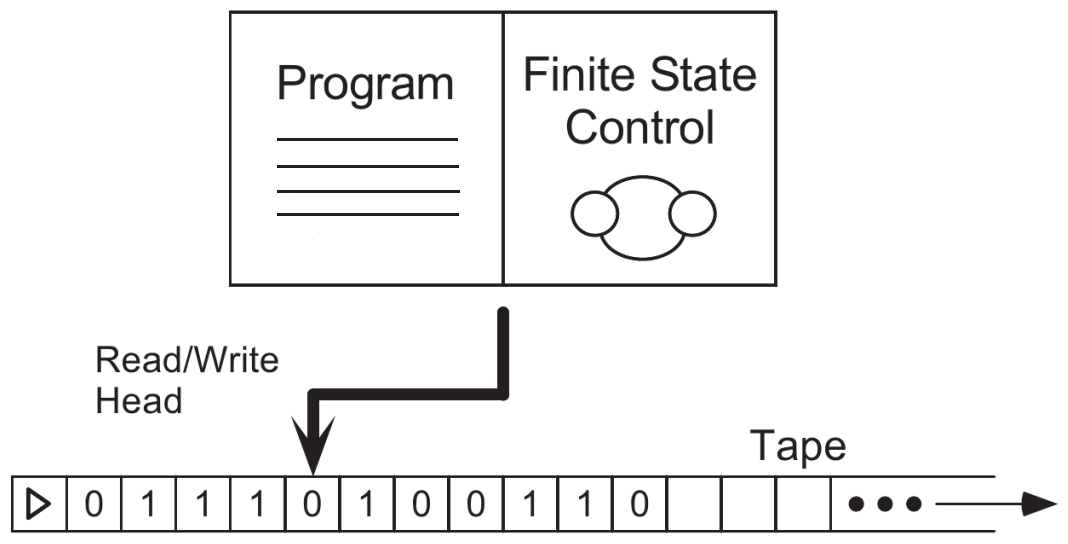
\includegraphics[width=8cm]{Images/Capitolo1/macchina_turing.png}
    \caption{Schema della Macchina di Turing.}
    \label{fig:macchina_turing}
\end{figure}
\newline
Ogni componente ha un suo scopo ben preciso: il controllo a stati finiti può essere paragonato ad un processore che può assumere un insieme finito di stati ($q_1, q_2, ..., q_m$); il nastro si può immaginare come una sequenza di caselle, ognuna delle quali conterrà un simbolo letto dalla stringa in input.

La testina può scorrere il nastro di una casella alla volta e agire su di essa di conseguenza.
Prima dell'esecuzione il controllo si troverà nello stato di partenza $q_i$ e la testina indicherà il simbolo $\rhd$ all'inizio del nastro.
Il programma, costituito da una quintupla di elementi, regola l'evoluzione dell'algoritmo.

Per prima cosa viene selezionata la stringa che ha come primo elemento lo stato in cui si trova il controllo e come secondo, il simbolo indicato dalla testina.
Se la stringa cercata non è presente nel programma la macchina assume lo stato di arresto $q_h$ e l'esecuzione del programma termina, in caso contrario la configurazione della macchina cambierà e verranno analizzati i tre elementi successivi.
Questi elementi rappresentano rispettivamente: lo stato che il controllo dovrà assumere, un simbolo di $\Gamma$ che la testina scrive sulla casella puntata e lo spostamento facoltativo della testina di una casella, a sinistra o a destra sul nastro.
Fino a quando la macchina non assume lo stato $q_h$ il ciclo prosegue, quando questo avviene l'output del programma sarà memorizzato nella casella su cui punta la testina.

La macchina di Turing che è stata presa in esame è la più semplice, altre varianti possono differire nel numero di nastri o nella loro dimensionalità, rimanendo tuttavia equivalenti.

Nella Figura \ref{fig:esempio_turing} viene mostrato un esempio di automa di macchina di Turing in grado risolvere il problema del riporto, o più semplicemente, di sommare 1 alla stringa di bit letta in input.
\newline
\begin{figure}[htp]
    \centering
    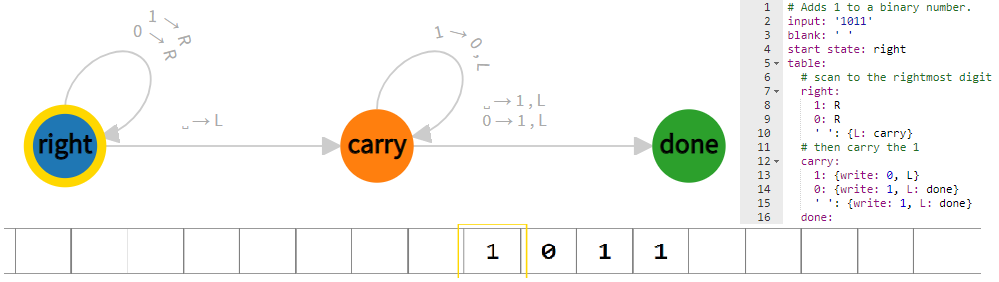
\includegraphics[width=11cm]{Images/Capitolo1/esempio_turing.png}
    \caption{Problema del riporto su Macchina di Turing.}
    \label{fig:esempio_turing}
\end{figure}

\section{I computer quantistici}
\textit{Il computer quantistico non si basa su un modello computazionale classico, utilizza piuttosto i principi della meccanica quantistica per la risoluzione di problemi che appartengono alle più svariate categorie. Tra queste troviamo la chimica quantistica e l'informatica quantistica, con tutte le loro sfaccettature \cite{hofmann2003articolo}.} 

Alla fine degli anni '70 la computazione classica probabilistica acquistò enorme importanza in ambito informatico e di conseguenza vennero implementati i primi algoritmi non deterministici, facendo così nascere dei dubbi sulla tesi di Church-Turing \cite{church1985articolo}.

Iniziò la ricerca di un modello computazionale in grado di simulare efficientemente qualsiasi altro modello computazionale.
La prima proposta di computer quantistico apparve nel 1959 grazie a Richard Feynman, in seguito, nel 1982 il fisico Paul Benioff \cite{quantum2001articolo} riuscì a dimostrare che la macchina di Turing classica poteva simulare certi fenomeni fisici senza incorrere in un rallentamento esponenziale delle sue prestazioni. Tre anni dopo David Deutsch \cite{hofmann2003articolo} ipotizzò che, essendo in definitiva le leggi della fisica approssimabili a quelle della meccanica quantistica, si potesse usare un dispositivo basato sui principi della meccanica quantistica per simulare efficientemente un sistema fisico arbitrario.

Le vere potenzialità di questa nuova scienza vennero messe in risalto nei primi anni Novanta da Richard Jozsa, il quale nel 1991, dopo aver descritto quali sono le funzioni che non possono essere risolte dal parallelismo quantistico, collaborò con Deutsch proponendo il primo problema che una macchina quantistica riusciva a risolvere in tempi più rapidi rispetto ad una deterministica.

La svolta epocale si ebbe nel 1994 con Peter Shor il quale pubblicò un algoritmo quantistico riuscendo a risolvere il problema della fattorizzazione di numeri molto grandi in un tempo polinomiale; due anni dopo Lov Grover scoprì la possibilità di trovare un record all'interno di un database in tempi più brevi rispetto agli algoritmi adottati nei computer classici \cite{algorithm2018articolo}.

Questi sviluppi portarono alla concezione odierna di computer quantistici: calcolatori che sfruttano le leggi della fisica e della meccanica quantistica con una capacità di calcolo, per alcune tipologie di problemi, di gran lunga superiore rispetto al computer classico.

Lo studio di queste macchine ha dato origine ad un nuovo settore della ricerca teorica nell'informatica e nella fisica che prende il nome di computazione quantistica, la quale stravolgerà completamente il trattamento dell'informazione, riuscendo a risolvere problemi scientifici attualmente irrisolvibili.

\subsection{Sviluppi nell'era moderna}
Tra la fine degli anni Novanta e i primi anni Duemila vennero condotti diversi esperimenti che diedero alla luce i primi computer quantistici, basati su un numero esiguo di qubit ($2\div 7$).
Questi esperimenti, effettuati nelle università di Stanford, Monaco e nel Laboratorio Nazionale di Los Alamos, riuscirono a svolgere gli algoritmi di Deutsch e Shor.

Successivamente ebbero luogo altre scoperte e furono dimostrate ulteriori teorie, mirate sia allo sviluppo della macchina quantistica sia ai campi scientifici correlati.

A seguito di questi sviluppi è stato possibile realizzare componenti fisiche fino ad ora inesistenti, in grado di contribuire alla costruzione del primo computer di questo genere e contemporaneamente vennero sperimentate le prime reti quantistiche.
La rete quantistica DARPA \cite{qnetwork2005articolo} fu una di queste e venne resa operativa nel 2003; nel 2005 gli scienziati del Max Planck Institute sono riusciti a realizzare un prototipo funzionante e nello stesso anno, venne annunciato il primo qubyte.

Nel 2007 fa la sua prima apparizione pubblica la D-Wave System, azienda che produce quello che viene considerato il primo computer quantistico adiabatico a 16qubit, definito in questo modo dato che ricorda le trasformazioni adiabatiche della termodinamica: un sistema scambia e riacquista calore per gradi e non tutto in un unico istante.
Il primo computer quantistico fu commercializzato nel 2011 e prese il nome di D-Wave One, costituito da 128qubit; insieme al suo successore D-Wave Two furono entrambi acquistati da Google in collaborazione con la NASA.

Tutto questo creò molto scalpore a livello accademico e scontri di idee: alcuni erano convinti delle sue potenzialità, mentre altri cercavano di dimostrare che non si trattava di vere e proprie macchine quantistiche, ma soltanto di macchine classiche che sfruttavano effetti quantistici per velocizzare i calcoli.

Alcune delle più grandi aziende in campo tecnologico come IBM e Google ne hanno capito l'importanza ed è per questo che puntano alla costruzione e allo sviluppo di queste macchine \cite{preskill2018articolo}.
